\documentclass[a4paper, 12pt]{report}
\usepackage{cmap} % поиск в PDF
\usepackage[T2A]{fontenc} % Кодировка
\usepackage[utf8]{inputenc} % Кодировка исходного текста
\usepackage[unicode, pdftex]{hyperref} % Для ссылок
\usepackage[english,russian]{babel} % Локализация и переносы
\usepackage{subcaption}
\captionsetup{compatibility=false}
\pagestyle{plain} % Для обозначения страниц справа снизу

\usepackage{graphicx}
\graphicspath{ {./images/} }

% Основная часть
\author{Автор: Булат Насыров}
\title{RFT\_CS \\ \footnotesize{\textit{Rocket fuel and trajectory computing system}}}
\date{\today}


\begin{document}
\maketitle

\tableofcontents{}
\clearpage
{\bfseries\Huge Предисловие}\\

\textrm{
    О чем будет идти речь, когда будем обсуждать ПО?\\
    Так же как любая метафора, описание программного обеспечения с точки зрения архитектуры может что-то скрыть, а что-то, наоборот, проявить; может обещать больше, чем давать, и давать больше, чем обещать. \\
    Оснавная привлекательность архитектуры - это структура. А структура - это то, что доминирует над парадигмами и суждениями в мире разработки ПО - компонентами, классами, функциями, модулями, слоями и службами, микро или макро. Но макроструктура многих программных систем часто пренебрегает убеждениями или пониманием - организация советских предприятий, невероятные небоскребы-башни (манареты) Дженга, достигающие облаков, археологические слои, залегающие в горной породе. Структура ПО не всегда интуитивно очевидна, как структура зданий.\\
    Здания имеют очевидную физическую структуру, независимо от материала, из которого они построены, от их высоты или ширины, от их назначения и от наличия или отсутствия архитектурных украшений. Их структура мало чем отличается - в значительной мере она обусловлена законом тяготения и физическими свойствами материалов. ПО, напротив, никак не связано с тяжестью, кроме чувства серьезности. И из чего же сделано ПО? В отличие от зданий, которые могут быть построены из кирпича, бетона, дерева, стали и стекла, программное обеспечение строится из меньших программных компонентов, и т.д., вплоть до основания.\\
    Говоря об архитектуре, можно сказать, что программное обеспечение по своей природе является фрактальным и рекурсивным, выгравированным и очерченным в коде. Здесь важные все детали. Переплетение уровней детализации также вносит свой вклад в архитектуру, но бессмысленно говорить о ПО в физических масштабах. Программное обеспечение имеет структуру - множество структур и множество их видов, - но их разнообразие затмевает диапазон физических структур, которые можно увидеть на примере зданий. Можно даже довольно убедительно утверждать, что при проектировании ПО архитектуре уделяется куда больше внимания, чем при проектировании зданий, - в этом смысле архитектура ПО является более многообразной, чем архитектура зданий!\\
    Но физический масштаб привычнее людям, и они часто ищут его в окружающем мире. Несмотря на привлекательность и визуальную очевидность, прямоугольники на диаграммах PowerPoint не являются архитектурой ПО. Да, они представляют определенный взгляд на архитектуру, значит не получить ни общей картины, ни понятия об архитектуре: архитектура ПО ни на что не похожа.
    Конкретный способ визуализации - не более чем частный выбор. Этот выбор основан на следующем наборе вариантов: что включить; что исключить; что подчеркнуть формой или цветом; что, наоборот, затенить. Никакой взгляд не имеет никаких преимуществ перед другим.\\
    Возможно, нет смысла говорить о законах физики и физических масштабах применительно к архитектуре ПО, но мы действительно учитываем некоторые физические ограничения. Скорость работы процессора и пропускная способность сети могут вынести суровый приговор производительности. Объем памяти и дискового пространства может ограничить амбиции любого программного кода. ПО можно сравнить с такой материей, как мечты, но ему приходится работать в реальном, физическим мире.\\
    \begin{quote}
        \textit{В любви, дорогая, чудовищна только безграничность воли, безграничность воли, безграничность желаний, несмотря на то, что силы наши ограничены, а осуществление мечты - в тисках возможности.}
    \end{quote}
    \begin{flushright}
        \citeA{Вильям Шекспир}
    \end{flushright}\\
    Физический мир – это мир, в котором мы живем, в котором находятся и действуют наши компании и экономика. Это дает нам другой подход к пониманию архитектуры программного обеспечения, позволяющий говорить и рассуждать не в терминах физических законов и понятий.
    \begin{quote}
        \textit{Архитектура отражает важные проектные решения по формированию системы, где важность определяется стоимостью изменений.}
    \end{quote}
    \begin{flushright}
        Гради Буч
    \end{flushright}\\
    Время, деньги, трудозатраты – вот еще одна система координат, помогающая нам различать большое и малое и отделять относящееся к архитектуре от всего остального. Она также помогает дать качественную оценку архитектуре – хорошая она или нет: хорошая архитектура отвечает потребностям пользователей, разработчиков и владельцев не только сейчас, но и продолжит отвечать им в будущем.
    \begin{quote}
        \textit{Если вы думаете, что хорошая архитектура стоит дорого, попробуйте плохую архитектуру.}
    \end{quote}
    \begin{flushright}
        Брайан Фут и Джозеф Йодер
    \end{flushright}
    Типичные изменения, происходящие в процессе разработки системы, не должны быть дорогостоящими, сложными в реализации; они должны укладываться в график развития проекта и в рамки дневных или недельных заданий.\\
    Это ведет нас прямиком к большой физической проблеме: путешествиям во времени. Как узнать, какие типичные изменения будут происходить, чтобы на основе этого знания принять важные решения? Как уменьшить трудозатраты и стоимость разработки без машины времени и гадания на кофейной гуще?\\
    \begin{quote}
        \textit{Архитектура – это набор верных решений, которые хотелось бы принять на ранних этапах работы над проектом, но которые не более вероятны, чем другие.}
    \end{quote}
    \begin{flushright}
        Ральф Джонсон
    \end{flushright}
    Анализ прошлого сложен; понимание настоящего в лучшем случае переменчиво; предсказание будущего нетривиально.\\
    К цели ведет много путей.\\
    На самом темном пути подстерегает мысль, что прочность и стабильность архитектуры зависят от строгости и жесткости. Если изменение оказывается слишком дорогостоящим, оно отвергается – его причины отменяются волевым решением. Архитектор имеет полную и безоговорочную власть, а архитектура превращается в антиутопию для разработчиков и постоянный источник недовольств.\\
    От другого пути исходит сильный запах спекулятивной общности. Он полон догадок, бесчисленных параметров, могильников с «мертвым» кодом и на нем подкарауливает множество случайных сложностей, способных покачнуть бюджет, выделенный на обслуживание.\\
    Но самый интересный – третий, чистый путь. Он учитывает природную гибкость программного обеспечения и стремится сохранить ее как основное свойство системы. Он учитывает, что мы оперируем неполными знаниями и, будучи людьми, неплохо приспособились к этому. Он играет больше на наших сильных сторонах, чем на слабостях. Мы создаем что-то и совершаем открытия. Мы задаем вопросы и проводим эксперименты. Хорошая архитектура основывается скорее на понимании движения к цели как непрерывного процесса исследований, а не на понимании самой цели как зафиксированного артефакта.\\
    \begin{quote}
        \textit{Архитектура – это гипотеза, которую требуется доказать реализацией и оценкой.}
    \end{quote}
    \begin{flushright}
        Том Гилб
    \end{flushright}
    Чтобы пойти по этому пути, нужно быть усердным и внимательным, нужно уметь думать и наблюдать, приобретать практические навыки и осваивать принципы. Сначала кажется, что это долгий путь, но в действительности все зависит от темпа вашей ходьбы.\\
    \begin{quote}
        \textit{Поспешай не торопясь.}
    \end{quote}
    \begin{flushright}
        Роберт С. Мартин
    \end{flushright}
    Получайте удовольствие от путешествия.
}

\chapter{Введение}
\section{Концепция}
\textrm{
    RFT\_CS (Rocket fuel and trajectory computing system) Система расчета ракетного топлива и траектории полета ракеты - это Python-библиотека для разработки математических моделей. RFT\_CS изначально был спроектирован так, чтобы его можно было внедрять постепенно. Другими словами, \textbf{вы можете начать с малого и использовать только ту функциональность RFT\_CS, которая необходима вам в данный момент}. Также в случае, если вам нужно изменить поведение/вычисления функции, есть возможность конфигурации методов под ваши нужды.
}
\section{Цель}
\textrm{
    Основная цель - создать математическую модель процессов, связанных с полётом одно и многоступенчатых, твердо и жидко топливных ракет и для вычисления траектории полёта баллистических ракет. Данное ПО может быть использовано для создания космических/баллистических ракет или своих научных экспериментов.
}
\section{Технологии}
\textrm{
    Программное обеспечение построено на высокоуровневом языке программирования Python и отдельные микропроцессоры написаны на языке C. Также для сложных математических вычислений использовались библиотеки, специально созданные для этой цели.
}
\clearpage

\section{Декомпозиция задачи}
\textrm{
    Начнём с составных частей ракеты, а также внешние факторы, влияющие на полёт. Начнём с состава космической ракеты:
}

\begin{figure}[!ht]
\centering
\begin{subfigure}
    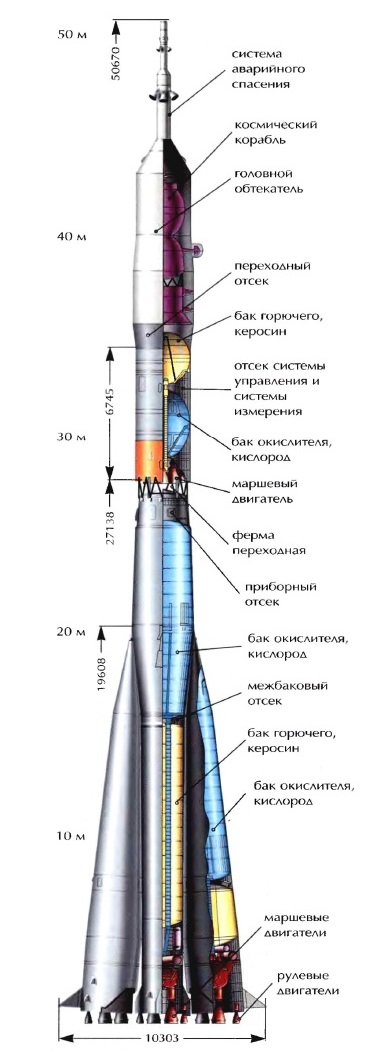
\includegraphics[width=.3\linewidth]{пример_космической_ракеты}
    \label{Рис. 1. Состав космической ракеты}
\end{subfigure}
\begin{subfigure}
    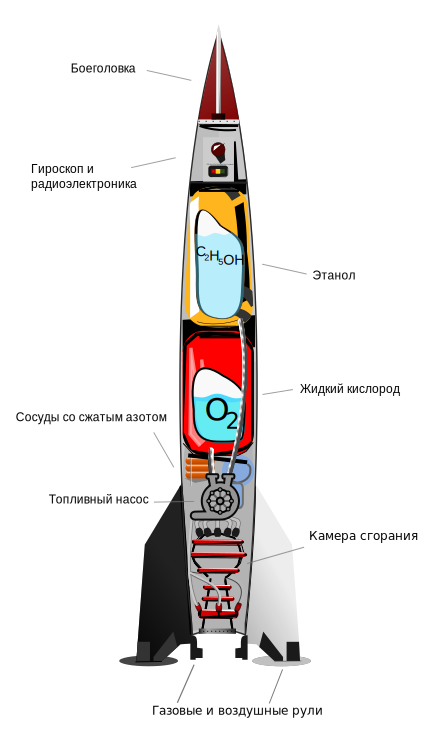
\includegraphics[width=.4\linewidth]{пример_баллистической_ракеты}
    \label{Рис. 2. Состав баллистической ракеты}
\end{subfigure}
\end{figure}

\section{Обработка ошибок}
\textrm{
    Могут возникать ошибки связанных с некорректным математических операций, перегрузкой или долгим ожиданием ответа от системы и неверным вводом/выводом данных, и др. Подобные ошибки обрабатываются и выводятся в виде ответа, а также записываются в логи. "{\bfseries При добавлении новых функций или использование встроенных функций важно не забывать обрабатывать ошибки и добавлять логирование для дальнейшего удобства исправления багов.}"
}
\clearpage
\chapter{Установка}
\section{Создание среды Linux/MacOS}
\textrm{
    Для создания виртуального окружения вам понадобиться установленный \href{https://python-poetry.org/}{Poetry\ldots}, \href{https://docs.python.org/3.9/}{Python версии 3.9}. После установки из GitHub, вы открываете рабочую директорию RFT\_CS. {\slshape poetry install}, после загрузки вы пишите\ldots {\slshape source .venv/bin/activate \Upsilon Супер виртуальная среда активирована!}\\
}
\section{Запуск программы Linux/MacOs}
\textrm{
    Чтобы запустить программу, вы должны зайти в директорию RFTCS \Rightarrow написать: {\slshape python3 main.py} и уже заполнять данные в формате целого или дробного числа.
}
\section{Создание среды Windows}
\textrm{
    Для создания виртуального окружения вам понадобиться установленный \href{https://python-poetry.org/}{Poetry\ldots}, \href{https://docs.python.org/3.9/}{Python версии 3.9}. После установки из GitHub, вы открываете рабочую директорию RFT\_CS. {\slshape poetry install}, после загрузки вы пишите\ldots {\slshape .venv\textbackslash Scripts \textbackslash activate \Upsilon Супер виртуальная среда активирована!}
}\\
\section{Запуск программы Windows}
\textrm {
    Чтобы запустить программу, вы должны зайти в директорию RFTCS написать: {\slshape python main.py} и уже заполнять данные в формате целого или дробного числа.
}
\section{Создание среды с использованием Makefile}
\textrm{
    Для этого достаточно перейти в директорию {\slshape .INSTALL/install\_env} и написать\ldots {\slshape make}
}
\clearpage
\chapter{Численное моделирование топлива ракеты}
\section{Описание}
\textit{Численное моделирование топлива ракеты. Производяться расчеты связанные с кольчеством топлива на разных стадиях топлива.}\\
\section{Импорты}
\textrm{Импортируется библиотеки numpy и matplotlib, и typing. Из файла format импортируется функция main\_rocket\_format, для более удобного вывода результа в консоль или json файл.}

\section{Классы}
\begin{itemize}
    \item TotalOil (Класс для расчета топлива) - принимает 3 параметра (масса пустой и полной ракеты, и Isp, с типом float). Включает функции:
    \begin{itemize}
        \item \_natural\_logarithm - (Скрытая функция получение натурального логарифма) - принимает 2 параметра (массу полной и пустой ракеты, с типом float).
        \item \_euler - (Скрытая функция расчет с помощью Эйлерова числа E) - принимает 1 параметр (общая скорость, с типом float).
        \item total\_speed - (Функция сумма всех скоростей) - принимает 2 параметра (натуральный логарифм и Isp, с типом float).
        \item total\_oil - (Функция для расчета топлива) - принимает 2 параметра (масса пустой ракеты и число эйлера, с типом float).
    \end{itemize}
\end{itemize}
\clearpage

\chapter{Расчет траектории полета ракеты}
\section{Описание}
\textit{Определяет траекторию полёта ракеты.}
\section{Импорты}
\begin{itemize}
    \item Импортируется библиотеки numpy и typing.
    \item Из файла rocket\_flight\_simulation импортируется функция resistance\_force\_env, для расчета лобового сопротивления.
    \item Из файла rocket\_fuel\_calculation импортируется функция total\_oil, для получения общего количества топлива в ракете.
\end{itemize}
\section{Константы}
\begin{itemize}
    \item Ускорение свободного падения
    \begin{itemize}
        \item 9.81
    \end{itemize}
    \item Угол вектора тяги над горизонтом, градусов
    \begin{itemize}
        \labelitemi 15
    \end{itemize}
\end{itemize}
\section{Классы}
\begin{itemize}
    \item FlightBallistics (Класс для расчета траектории полета {\itseries внутри Земли}) - принимает 1 параметр (скорость, с типом float). Включает функции:
    \begin{itemize}
        \item \_double\_angle\_sine (Скрытая функция расчета синуса двойного угла) - принимает 1 параметр и 1 константу (скорость ракеты и угол вектора тяги над горизонтом, с типом float), выводит число типа float.
        \item flight\_range (Функция дальности полета) - принимает 2 параметра и 2 константы (ускорение свободного полета, угол вектора тяги над горизонтом, синус двойного угла и скорость, с типом float), выводит число типа float.
        \item flight\_time (Функция время полета ракеты) - принимает 1 параметр и 2 константы (ускороние свободного полета, угол двойного угла и скорость, всё с типом float), выводит число типа float.
    \end{itemize}
\end{itemize}
\clearpage

\chapter{Численное моделирование полета ракеты}
\section{Описание}
\textit{Численное моделирование полета ракеты. Производяться расчеты связанные с полётом ракеты в земной среде. Используются физические явления: поступательное и вращательное движение; гравитация; зависимость плотности воздуха от высоты; реактивная сила с отклонением вектором тяги; сопротивления воздуха.}
\section{Импорты}
\begin{itemize}
    \item Из файла rocket\_fuel\_calculation.py импортируется функция total\_speed, для получения дельта скорости (общей скорости).
    \item Из файла format импортируется класс FlightFormat, для более удобного вывода результа в консоль.
\end{itemize}
\section{Константы}
\begin{itemize}
    \item Плотность воздуха, кг/м^{3} - 1.27
    \item Молярная масса, кг/моль - 0.029
    \item Температура, K - 300
    \item Ускорение свободного падения - 9.81
    \item Ро - плотность - 16900
    \item Коэфициент формы - 1.2
    \item Коэффициент лобового сопротивления - 0.14
\end{itemize}
\section{Функции}
\begin{itemize}
    \item distance\_N\_step (Функция расстояния от горящей поверхности топлива до стенки камеры сгорания) - принимает 2 параметра (расход топлива и шаг, с типом float), выводи число типа float.
    \item tg\_Beta (Функция угол полета ракеты относительно поверности земли) - принимает 1 параметр и 2 константы (скорость, радиус земли и начальный радиус старта ракеты, с типом float), выводит число типа float.
    \item elliptical\_range (Функция эллиптической дальности полета) - принимает 1 параметр и 1 константу (скорость и радиус Земли, с типом float), выводит число типа float.
    \item mass\_rocket (Функция массы ракеты) - принимает 2 параметра (масса пустой ракеты и топлива ракеты, с типом float), выводит число типа float.
    \item amount\_gas\_released (Функция количества выделяемого газа за 1 моль) - принимает 1 параметр и 1 константу (масса и средняя молярная масса, с типом float), выводит число типа float.
    \item overpressure (Функция избыточного давления в камере сгорания на n-шаге) - принимает 1 параметр и 3 константы (расход, средняя молярная масса, универсальная газовая константа и температура горения, с типом float), выводит число типа float.
    \item thrust\_force (Функция силы тяги) - принимает 1 параметр и 1 константу (давление и площадь поперечного сечения, с типом float), выводит число типа float.
    \item impuls (Функция импульса, сообщаемого ракете на n-шаге), принимает 2 параметра (давление и время, с типом float), выводит число типа float.
    \item height\_force (Функция высоты ракеты над стартовой площадкой) - принимает 3 параметра (высота площадки, высота ступени, количество ступеней, с типом float), выводит число типа float.
\end{itemize}
\section{Классы}
\begin{itemize}
    \item Resistance (Класс для расчета сопротивления) - принимает 3 параметра (скорость, сила тяги и масса, с типом float). Включает функции:
        \begin{itemize}
            \item \_aerodynamic\_pressure (Скрытая функция аэродинамического напора) - принимает 1 параметр и 1 константу (скорость и плотность воздуха, с типом float), выводит число с типом float.
            \item aerodynamic\_drag (Функция аэродинамического сопротивления) - принимает 1 параметр и 1 константу (аэродинамическое сопротивление и площадь поперечного сечения, с типом float), выводит число типа float.
            \item gravitation\_losses (Функция гравитационные потери) - принимает 2 константы (ускорение свободного падения и угол вектора тяги над горизонтом, с типом float), выводит число типа float.
            \item control\_losses (Функция потери скорости на управление) - принимает 2 параметра и 1 константу (сила тяги, массу и угол между векторами тяги, и скорости ракеты, с типом float), выводит число типа float.
        \end{itemize}
    \item Speed (Класс для расчета скорости) - принимает 5 параметров (силу тяги, гравитционные потери, масса, время, начальная скорость, с типом float). Включает функции:
        \begin{itemize}
            \item \_resultant\_force (Скрытая функция равнодействующая сила) - принимает 3 параметра и 1 константу (силу тяги, гравитационное сопротивления, массу и ускорение свободного падения, с типом float), выводит число типа float.
            \item rocket\_acceleration (Функция ускорение ракеты) - принимает 2 параметр (равнодействующая сила и масса, с типом float), выводит число типа float.
            \item rocket\_speed (Функция скорости ракеты) - принимает 3 параметра (начальная скорость, ускорение ракеты и время, с типом float), выводит число типа float.
        \end{itemize}
    \item ModelFlight (Класс для моделирования полета) - принимает 4 параметра (масса, начальная скорость, время и сила тяги, с типом float). Включает функции:
        \begin{itemize}
            \item \_total\_resistance (Скрытая функция сумма сопротивлений), принимает 4 параметра (скорость, сила тяги, масса, с типом float), выводит число типа float.
            \item \_total\_speed (Скрытая функция сумма скоростей), принимает 5 параметров (сила тяги, гравитационное сопротивление, масса, время, начальная скорость, с типом float), выводит типа float.
            \item \_total\_distance (Скрытая функция общая дистанция), принимает 1 параметр (общая скорость, с типом float), выводит с типа float.
            \item model\_stack (Функция списка параметров), принимает 3 параметра (сумма сопротивлений, сумма скоростей и общая дистанция, с типом float), выводит 4 значения (сопротивление, скорость, расстояние, угол полета ракеты) с типами float.
        \end{itemize}
\end{itemize}

\end{document}

